\begin{figure}[h]
    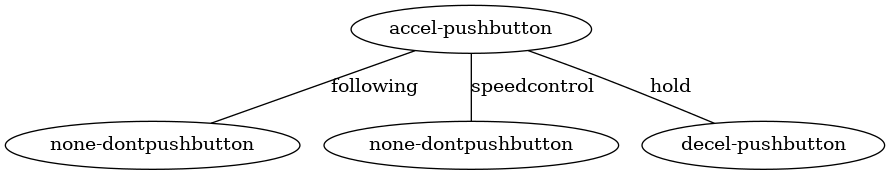
\includegraphics[width=\textwidth]{result-figs/ACC-minstandby-scen4_hum.png}
    \caption{Human Policy for Scenario 2 starting in Standby}
    \label{fig:standby-s4-hum}
\end{figure}

\begin{figure}[h]
    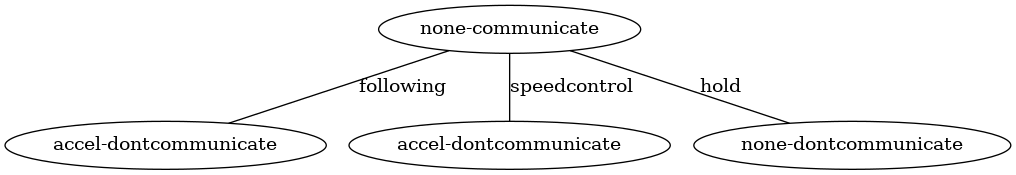
\includegraphics[width=\textwidth]{result-figs/ACC-minstandby-scen4_mach.png}
    \caption{Machine Policy for Scenario 2 starting in Standby}
    \label{fig:standby-s4-mach}
\end{figure}

\begin{figure}[h]
    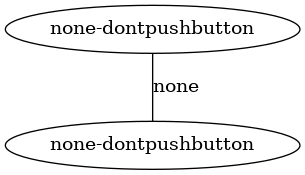
\includegraphics[width=\textwidth]{result-figs/ACC-minfollowing-scen4_hum.png}
    \caption{Human Policy for Scenario 2 starting in Standby}
    \label{fig:following-s4-hum}
\end{figure}

\begin{figure}[h]
    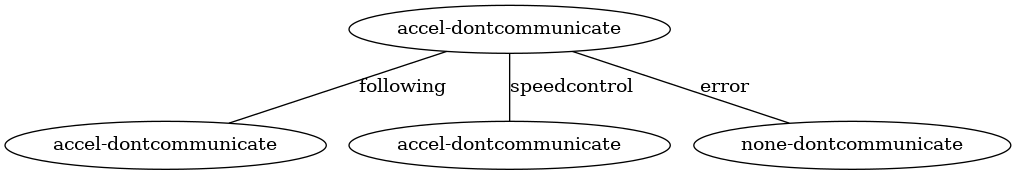
\includegraphics[width=\textwidth]{result-figs/ACC-minfollowing-scen4_mach.png}
    \caption{Machine Policy for Scenario 2 starting in Standby}
    \label{fig:following-s4-mach}
\end{figure}

\begin{figure}[h]
    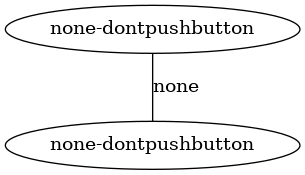
\includegraphics[width=\textwidth]{result-figs/ACC-minspeedcontrol-scen4_hum.png}
    \caption{Human Policy for Scenario 2 starting in Standby}
    \label{fig:speedcontrol-s4-hum}
\end{figure}

\begin{figure}[h]
    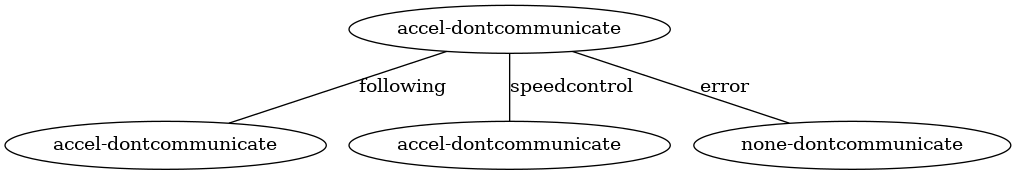
\includegraphics[width=\textwidth]{result-figs/ACC-minspeedcontrol-scen4_mach.png}
    \caption{Machine Policy for Scenario 2 starting in Standby}
    \label{fig:speedcontrol-s4-mach}
\end{figure}

\begin{figure}[h]
    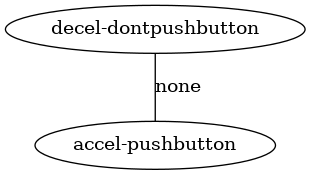
\includegraphics[width=\textwidth]{result-figs/ACC-minerror-scen4_hum.png}
    \caption{Human Policy for Scenario 2 starting in Standby}
    \label{fig:error-s4-hum}
\end{figure}

\begin{figure}[h]
    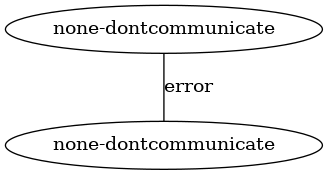
\includegraphics[width=\textwidth]{result-figs/ACC-minerror-scen4_mach.png}
    \caption{Machine Policy for Scenario 2 starting in Standby}
    \label{fig:error-s4-mach}
\end{figure}

\begin{figure}[h]
    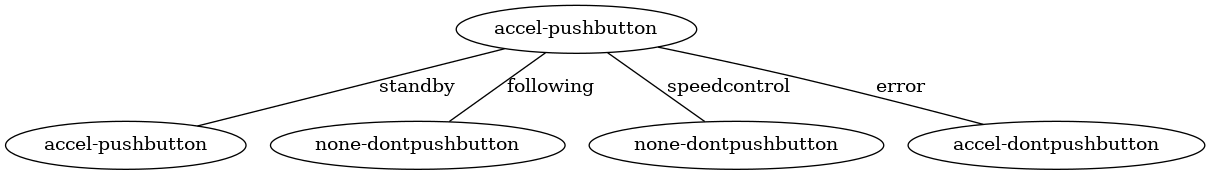
\includegraphics[width=\textwidth]{result-figs/ACC-minhold-scen4_hum.png}
    \caption{Human Policy for Scenario 2 starting in Standby}
    \label{fig:hold-s4-hum}
\end{figure}

\begin{figure}[h]
    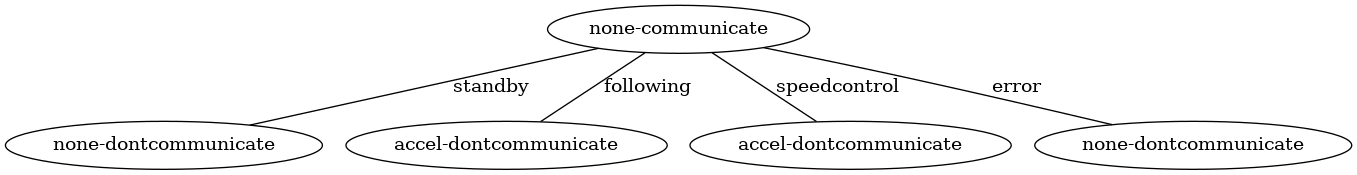
\includegraphics[width=\textwidth]{result-figs/ACC-minhold-scen4_mach.png}
    \caption{Machine Policy for Scenario 2 starting in Standby}
    \label{fig:hold-s4-mach}
\end{figure}

\begin{figure}[h]
    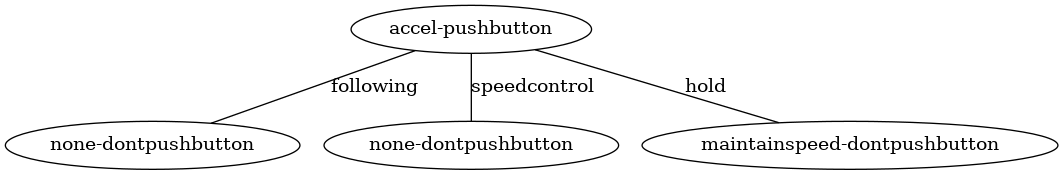
\includegraphics[width=\textwidth]{result-figs/ACC-minstandby-scen5_hum.png}
    \caption{Human Policy for Scenario 2 starting in Standby}
    \label{fig:standby-s5-hum}
\end{figure}

\begin{figure}[h]
    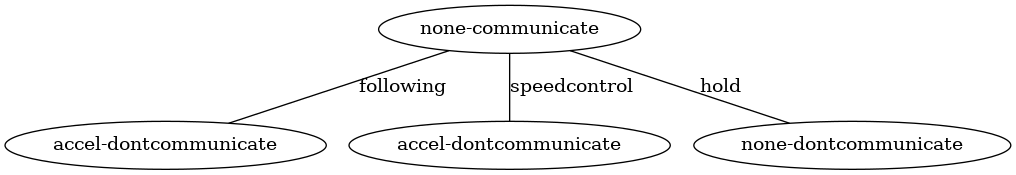
\includegraphics[width=\textwidth]{result-figs/ACC-minstandby-scen5_mach.png}
    \caption{Machine Policy for Scenario 2 starting in Standby}
    \label{fig:standby-s5-mach}
\end{figure}

\begin{figure}[h]
    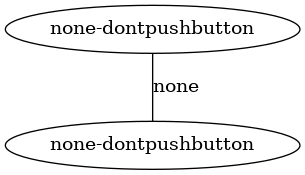
\includegraphics[width=\textwidth]{result-figs/ACC-minfollowing-scen5_hum.png}
    \caption{Human Policy for Scenario 2 starting in Standby}
    \label{fig:following-s5-hum}
\end{figure}

\begin{figure}[h]
    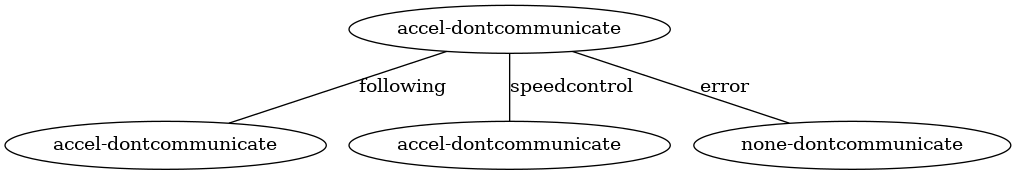
\includegraphics[width=\textwidth]{result-figs/ACC-minfollowing-scen5_mach.png}
    \caption{Machine Policy for Scenario 2 starting in Standby}
    \label{fig:following-s5-mach}
\end{figure}

\begin{figure}[h]
    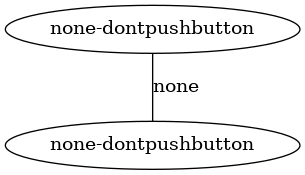
\includegraphics[width=\textwidth]{result-figs/ACC-minspeedcontrol-scen5_hum.png}
    \caption{Human Policy for Scenario 2 starting in Standby}
    \label{fig:speedcontrol-s5-hum}
\end{figure}

\begin{figure}[h]
    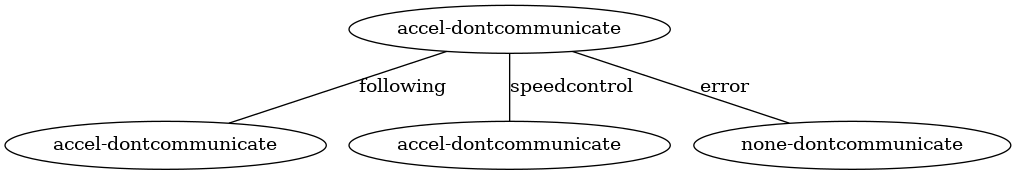
\includegraphics[width=\textwidth]{result-figs/ACC-minspeedcontrol-scen5_mach.png}
    \caption{Machine Policy for Scenario 2 starting in Standby}
    \label{fig:speedcontrol-s5-mach}
\end{figure}

\begin{figure}[h]
    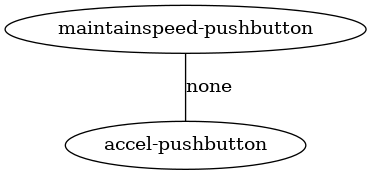
\includegraphics[width=\textwidth]{result-figs/ACC-minerror-scen5_hum.png}
    \caption{Human Policy for Scenario 2 starting in Standby}
    \label{fig:error-s5-hum}
\end{figure}

\begin{figure}[h]
    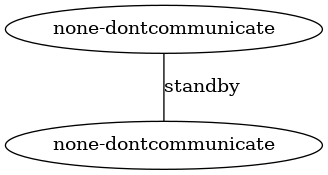
\includegraphics[width=\textwidth]{result-figs/ACC-minerror-scen5_mach.png}
    \caption{Machine Policy for Scenario 2 starting in Standby}
    \label{fig:error-s5-mach}
\end{figure}

\begin{figure}[h]
    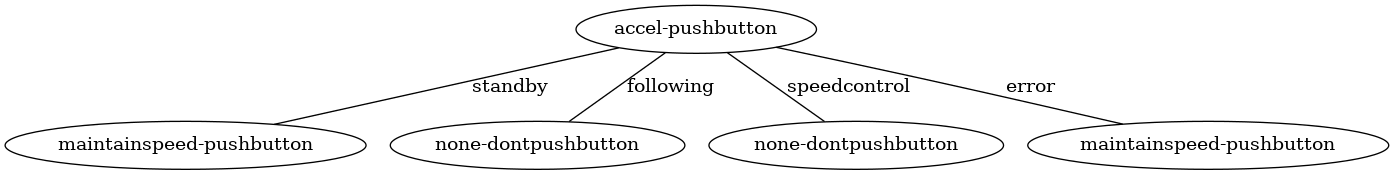
\includegraphics[width=\textwidth]{result-figs/ACC-minhold-scen5_hum.png}
    \caption{Human Policy for Scenario 2 starting in Standby}
    \label{fig:hold-s5-hum}
\end{figure}

\begin{figure}[h]
    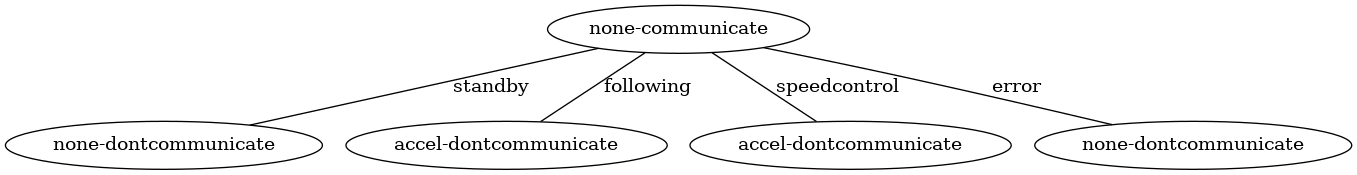
\includegraphics[width=\textwidth]{result-figs/ACC-minhold-scen5_mach.png}
    \caption{Machine Policy for Scenario 2 starting in Standby}
    \label{fig:hold-s5-mach}
\end{figure}

\begin{figure}[h]
    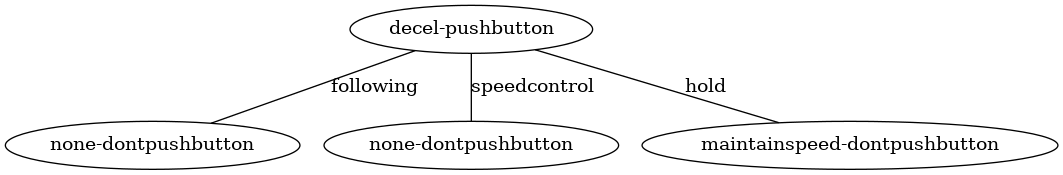
\includegraphics[width=\textwidth]{result-figs/ACC-minstandby-scen6_hum.png}
    \caption{Human Policy for Scenario 2 starting in Standby}
    \label{fig:standby-s6-hum}
\end{figure}

\begin{figure}[h]
    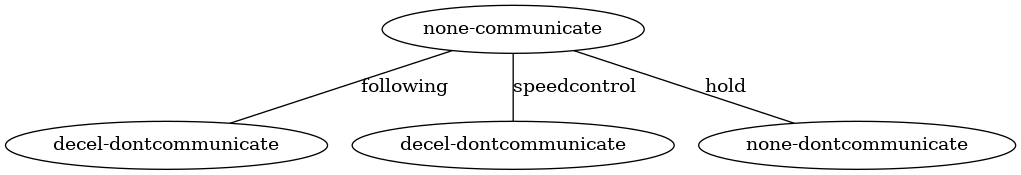
\includegraphics[width=\textwidth]{result-figs/ACC-minstandby-scen6_mach.png}
    \caption{Machine Policy for Scenario 2 starting in Standby}
    \label{fig:standby-s6-mach}
\end{figure}

\begin{figure}[h]
    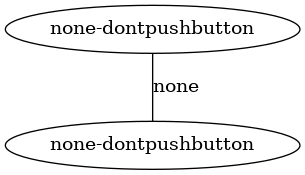
\includegraphics[width=\textwidth]{result-figs/ACC-minfollowing-scen6_hum.png}
    \caption{Human Policy for Scenario 2 starting in Standby}
    \label{fig:following-s6-hum}
\end{figure}

\begin{figure}[h]
    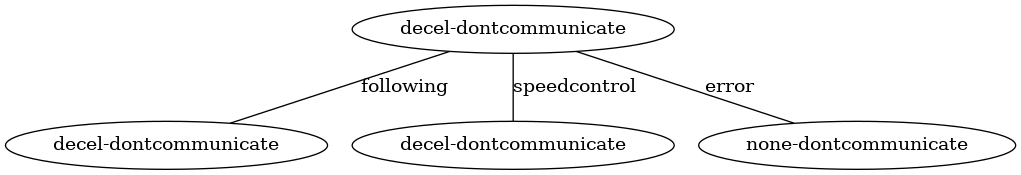
\includegraphics[width=\textwidth]{result-figs/ACC-minfollowing-scen6_mach.png}
    \caption{Machine Policy for Scenario 2 starting in Standby}
    \label{fig:following-s6-mach}
\end{figure}

\begin{figure}[h]
    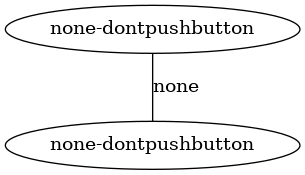
\includegraphics[width=\textwidth]{result-figs/ACC-minspeedcontrol-scen6_hum.png}
    \caption{Human Policy for Scenario 2 starting in Standby}
    \label{fig:speedcontrol-s6-hum}
\end{figure}

\begin{figure}[h]
    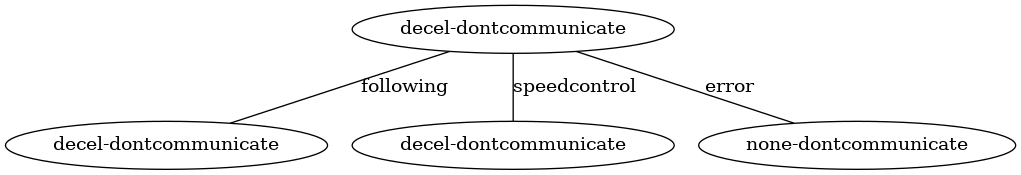
\includegraphics[width=\textwidth]{result-figs/ACC-minspeedcontrol-scen6_mach.png}
    \caption{Machine Policy for Scenario 2 starting in Standby}
    \label{fig:speedcontrol-s6-mach}
\end{figure}

\begin{figure}[h]
    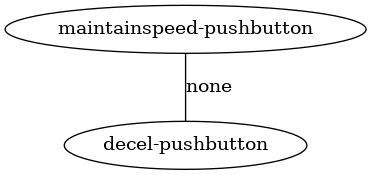
\includegraphics[width=\textwidth]{result-figs/ACC-minerror-scen6_hum.png}
    \caption{Human Policy for Scenario 2 starting in Standby}
    \label{fig:error-s6-hum}
\end{figure}

\begin{figure}[h]
    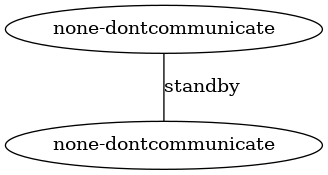
\includegraphics[width=\textwidth]{result-figs/ACC-minerror-scen6_mach.png}
    \caption{Machine Policy for Scenario 2 starting in Standby}
    \label{fig:error-s6-mach}
\end{figure}

\begin{figure}[h]
    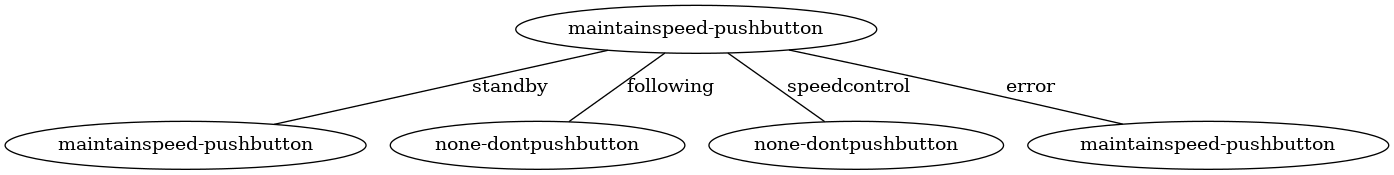
\includegraphics[width=\textwidth]{result-figs/ACC-minhold-scen6_hum.png}
    \caption{Human Policy for Scenario 2 starting in Standby}
    \label{fig:hold-s6-hum}
\end{figure}

\begin{figure}[h]
    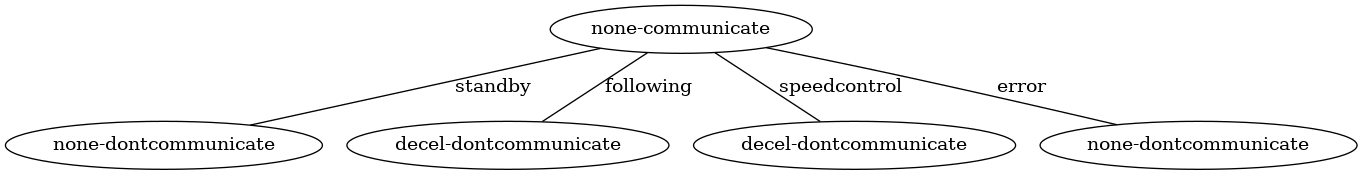
\includegraphics[width=\textwidth]{result-figs/ACC-minhold-scen6_mach.png}
    \caption{Machine Policy for Scenario 2 starting in Standby}
    \label{fig:hold-s6-mach}
\end{figure}

\begin{figure}[h]
    \includegraphics[width=\textwidth]{result-figs/ACC-minstandby-scen7_hum.png}
    \caption{Human Policy for Scenario 2 starting in Standby}
    \label{fig:standby-s7-hum}
\end{figure}

\begin{figure}[h]
    \includegraphics[width=\textwidth]{result-figs/ACC-minstandby-scen7_mach.png}
    \caption{Machine Policy for Scenario 2 starting in Standby}
    \label{fig:standby-s7-mach}
\end{figure}

\begin{figure}[h]
    \includegraphics[width=\textwidth]{result-figs/ACC-minfollowing-scen7_hum.png}
    \caption{Human Policy for Scenario 2 starting in Standby}
    \label{fig:following-s7-hum}
\end{figure}

\begin{figure}[h]
    \includegraphics[width=\textwidth]{result-figs/ACC-minfollowing-scen7_mach.png}
    \caption{Machine Policy for Scenario 2 starting in Standby}
    \label{fig:following-s7-mach}
\end{figure}

\begin{figure}[h]
    \includegraphics[width=\textwidth]{result-figs/ACC-minspeedcontrol-scen7_hum.png}
    \caption{Human Policy for Scenario 2 starting in Standby}
    \label{fig:speedcontrol-s7-hum}
\end{figure}

\begin{figure}[h]
    \includegraphics[width=\textwidth]{result-figs/ACC-minspeedcontrol-scen7_mach.png}
    \caption{Machine Policy for Scenario 2 starting in Standby}
    \label{fig:speedcontrol-s7-mach}
\end{figure}

\begin{figure}[h]
    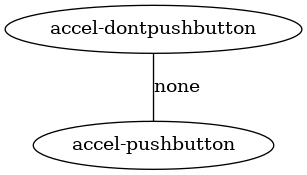
\includegraphics[width=\textwidth]{result-figs/ACC-minerror-scen7_hum.png}
    \caption{Human Policy for Scenario 2 starting in Standby}
    \label{fig:error-s7-hum}
\end{figure}

\begin{figure}[h]
    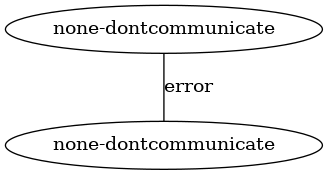
\includegraphics[width=\textwidth]{result-figs/ACC-minerror-scen7_mach.png}
    \caption{Machine Policy for Scenario 2 starting in Standby}
    \label{fig:error-s7-mach}
\end{figure}

\begin{figure}[h]
    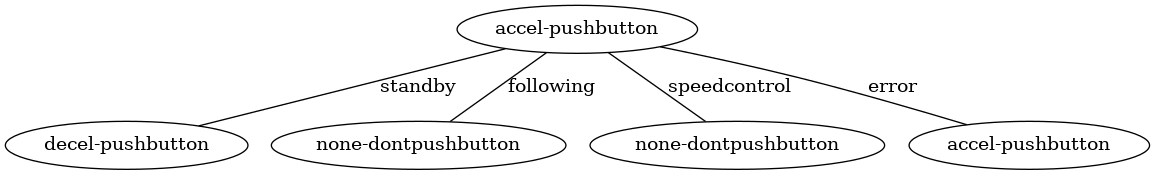
\includegraphics[width=\textwidth]{result-figs/ACC-minhold-scen7_hum.png}
    \caption{Human Policy for Scenario 2 starting in Standby}
    \label{fig:hold-s7-hum}
\end{figure}

\begin{figure}[h]
    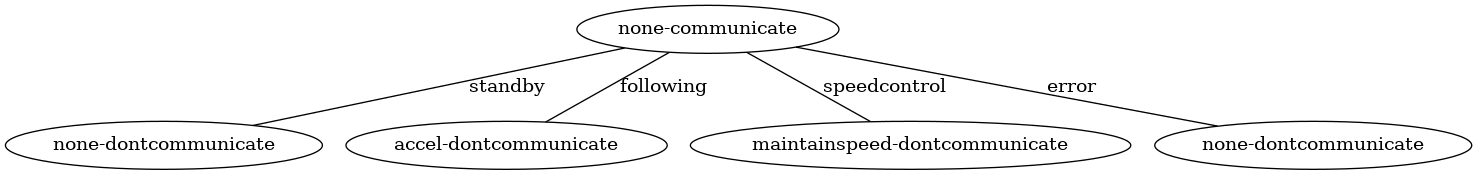
\includegraphics[width=\textwidth]{result-figs/ACC-minhold-scen7_mach.png}
    \caption{Machine Policy for Scenario 2 starting in Standby}
    \label{fig:hold-s7-mach}
\end{figure}

